%%%%%%%%%%%%%%%%%%%%%%%%%%%%%%%%%%%%%%%%%
% Journal Article
% LaTeX Template
% Version 1.3 (9/9/13)
%
% This template has been downloaded from:
% http://www.LaTeXTemplates.com
%
% Original author:
% Frits Wenneker (http://www.howtotex.com)
%
% License:
% CC BY-NC-SA 3.0 (http://creativecommons.org/licenses/by-nc-sa/3.0/)
%
%%%%%%%%%%%%%%%%%%%%%%%%%%%%%%%%%%%%%%%%%

%----------------------------------------------------------------------------------------
%	PACKAGES AND OTHER DOCUMENT CONFIGURATIONS
%----------------------------------------------------------------------------------------

\documentclass[twoside]{article}

\usepackage{lipsum} % Package to generate dummy text throughout this template

\usepackage[sc]{mathpazo} % Use the Palatino font
\usepackage[T1]{fontenc} % Use 8-bit encoding that has 256 glyphs
\linespread{1.05} % Line spacing - Palatino needs more space between lines
\usepackage{microtype} % Slightly tweak font spacing for aesthetics
\usepackage{paralist}
\usepackage[margin={1.5cm,1.5cm},top=32mm,columnsep=20pt]{geometry} % Document margins
\usepackage{multicol} % Used for the two-column layout of the document
\usepackage[hang, small,labelfont=bf,up,textfont=it,up]{caption} % Custom captions under/above floats in tables or figures
\usepackage{booktabs} % Horizontal rules in tables
\usepackage{graphicx,float}
\usepackage{float} % Required for tables and figures in the multi-column environment - they need to be placed in specific locations with the [H] (e.g. \begin{table}[H])
\usepackage{hyperref} % For hyperlinks in the PDF
\usepackage{amsmath,amsfonts,amsthm}
\usepackage{lettrine} % The lettrine is the first enlarged letter at the beginning of the text
\usepackage{paralist} % Used for the compactitem environment which makes bullet points with less space between them
\usepackage{subfigure}% For side by side figure

\usepackage{abstract} % Allows abstract customization
\renewcommand{\abstractnamefont}{\normalfont\bfseries} % Set the "Abstract" text to bold
\renewcommand{\abstracttextfont}{\normalfont\small\itshape} % Set the abstract itself to small italic text
\usepackage[toc,page]{appendix}

\usepackage{algorithm}
\usepackage[noend]{algpseudocode}
\makeatletter
\def\BState{\State\hskip-\ALG@thistlm}
\makeatother

\usepackage{titlesec} % Allows customization of titles
\renewcommand\thesection{\arabic{section}} % Roman numerals for the sections
\renewcommand\thesubsection{\arabic{subsection}} % Roman numerals for subsections
\titleformat{\section}[block]{\Large\scshape\centering}{\thesection.}{1em}{} % Change the look of the section titles
\titleformat{\subsection}[block]{\large}{\thesection.\thesubsection.}{1em}{} % Change the look of the section titles

\usepackage{fancyhdr} % Headers and footers
\pagestyle{fancy} % All pages have headers and footers
\fancyhead{} % Blank out the default header
\fancyfoot{} % Blank out the default footer
\fancyhead[C]{Whales Recognition using Part One-vs-One Features} % Custom header text
\fancyfoot[RO,LE]{\thepage} % Custom footer text

%----------------------------------------------------------------------------------------
%	TITLE SECTION
%----------------------------------------------------------------------------------------

\title{\vspace{-15mm}\fontsize{24pt}{10pt}\selectfont\textbf{Whales Recognition using Part One-vs-One Features}} % Article title

\author{
\large
\textsc{Nicolas Drizard}\\[2mm] % Your name
\normalsize Final Project for CS283, Harvard University \\ % Your institution
\normalsize {nicolas.drizard@g.harvard.edu} % Your email address
\vspace{-5mm}
}
\date{}

%----------------------------------------------------------------------------------------

\begin{document}

\maketitle % Insert title

\thispagestyle{fancy} % All pages have headers and footers

%----------------------------------------------------------------------------------------
%	ABSTRACT
%----------------------------------------------------------------------------------------

\begin{abstract}

\noindent

Object recognition problems are divided in two different parts: instance recognition and class recognition. Whereas the first one correponds to find a specific object in an image, I decided to tackle the second one, also know as category-level recognition, where the objective is to recognize any instance of a particular general class. I implemented the Part One-vs-One Features (PooF) method developped in \cite{poof} for fine-grained recognition. This methods learns automatically a large and diverse set of features specialized in the discrimination between 2 particular classes based on the appearance at a particular part. I applied it on the CUB birds dataset \cite{cub} and on a whales data set to take part to a Kaggle competition \cite{kag}. The results obtained are very promising.

\end{abstract}

%----------------------------------------------------------------------------------------
%	ARTICLE CONTENTS
%----------------------------------------------------------------------------------------

\begin{multicols}{2} % Two-column layout throughout the main article text

\section{Introduction}

\lettrine[nindent=0em,lines=1]{K}aggle and the Northeast Fisheries Science Center currently host a competition to automatically recognise whales on aerial picture. The main motivation is that with fewer than 500 North Atlantic right whales left in the world's oceans, knowing the health and status of each whale is integral to the efforts of researchers working to protect the species from extinction. It appears that the different whales are very similar to each other on the picture and barely distinguishable with the naked eye.  As a result, I choose to implement the POOF to extract highly discriminative features from the images.\\

In this paper, I present the related work around this method and other available alternative to solve this kind of problem. Then, I developp in details how to build the Poofs and explain my implementation choices. The results of my experiments on two datasets follow, on a birds dataset \cite{cub} and on the whales dataset \cite{kag}. Lastly, I suggest further possible improvements after the presentation of the remaining challenges.


\section{Related Work}

Many instance recognition problems concern the human detection, a known dataset is the pedestrian one from MIT. A thorough study showed experimentally that grids of HOGs descriptors outperfomr largely other common features used in \cite{pedes}. The idea of the method is that the distribution of local edge direction is a sufficiant descriptor of an object shape, even whithout knowing in details the edge positions. This assess the use of these features in the Poof approach.\\

Another common method on object recognition is training Deformable Part Models (DPM). This work \cite{dpm} proposes a computationally-efficient method for to different pose-normalized descriptors. Pose- normalization was proposed for fine-grained recognition in \cite{birdlets}. This paradigm seeks to discount variations in pose, articulation and camera viewing angle by localizing semantic object parts and extracting appearance features with respect to those localized parts. It was first proposed using a computationnally-expensive method using Poselets.\\

Recently, many approaches were built taking advantage of Convolutionnal Neural Networks. These methods are computationally expensive but do not require any inputs except the labels. With only category labels as inputs, a method using bilinear CNN \cite{cnn} reached 84.1\% of accuracy in the CUB-200-2011 dataset \cite{cub}. A parts-based model is developped in \cite{cnn1} without the need for a bounding box. A similar method should be implemented in future work because it solves the issue of part annotation. Nonethelless, we chose to implement the Poof approach relying on the assumption that specific interests points on the nose of the whales are known, the issue is to developp a robust method to find them. 

\section{POOF Method}

In this part, I explain the different steps of the poof method developped in \cite{poof} with the same notations. The process requires as input a dataset with images labeled by class and annotated with part locations. It is nonetheless not necessary that all the parts be annotated in all the images. The output of the method is a set of highly discriminative features that we will use for a categoy-level classification task. Given a train set, the learning process is fully automatic.\\

Each POOF learned by the method is defined by:

\begin{compactitem}
	\item a tuple of two different classes $i,j \in {1,..., N}$ with $i<j$ (the roles are symmetric);
	\item one seed part for feature extraction $f \in {1,..., P}$;
	\item one other part for alignement; $a \in {1, ..., P}$, with $a \neq f$;
	\item a low level feature which can be extracted from a window. We use in the current implementation the histogram of oriented gradient which describes the local distribution of edge direction.
\end{compactitem}


We write $T^{i,j}_{f,a}$ for the Poof built on the presented configuration. This function assigns a single scalar score for any image in the domain. Each feature is learned following this procedure

\begin{enumerate}
	\item We consider the train images of classes $i$ and $j$ with the parts $f$ and $a$ visible. We perform a similarity transformation to bring points f and a to fixed position and crop the image to a rectangular region enclosing the two parts with a fixed size.
	\item We tile the croped images with a grid of feature cells for different scalse. For each tiling, we compute and extract the base feature for each cell.
	\item For the tiling at each scale, we train a linear support vector machine (SVM) to distinguish the two classes based on the concatenation of the base features over the grid.
	\item For each tiling, we extract from the trained SVM the weights assigned to each cell and keep the maximum value. Then, we applied a median thresholding to come up with a mask on the tiling with only half of the cells. Starting from the seed part $f$, we keep the connected component from the previous mask as the final mask. This defines a discriminative region around f for the classes $i$ and $j$.
	\item We concatenate over all the tilings the low level features computed on the cell from the masked image. We train a final linear SVM which learns a projection of the multiscale and local features to a single dimension. This projection is $T^{i,j}_{f,a}$.
\end{enumerate}

\section{Approach}

I chose to developp an end-to-end process applicable for any kind of category-level classification problem as long as there is labeled train images and that the whole dataset is annotated. This latter condition is not verified with the whales dataset, I had to annotate some pictures for my experiments. I will discuss this issue later.\\

The workflow is the following:
\begin{enumerate}
	\item Feature Extraction: we learn the Poof algorithm on the train images by computing for each configuration $(i, j, f, a)$ the tuple (mask, final svm) which defines $T^{i,j}_{f,a}$.
	\item On the whole dataset to consider (train and test), we extract the Poofs by applying the final svm on the concatenation of the HOG features of the masked croped image over the grids.
	\item We  train and apply on the test set one-vs-all classifiers for each class. We rank the different classes on each test image and assign to it the most likely.
\end{enumerate}

\section{Implementation Details}

In my implementation, We made the following choices (mostly inspired by \cite{poof}):

\begin{compactitem}
	\item In the alignement, We use a 64 pixel tall and 18 pixel wide rectangular box with the two parts placed on a horizontal line with 64 pixels between them.
	\item Before applying the similarity, We applied an axial symmetry against the vertical for the images where the part f was on the right of the part a. This enables to have all the croped images with the same local geometry. The effect is illustrated in the figure \ref{fig:fig_sym}. The image in the upper part is the one without a symmetry.
	\item We use two scales of grid for the base feature extraction, with 8 x 8 and 16 x 16 pixels.
	\item We use the histogramm of oriented gradient (HOG) as low level features. We used the implementation provided by vlfeat \cite{vlf}.  It decomposes the image into square cells of a given size, computes a histogram of oriented gradient from the algorithm of  Felzenswalb \cite{fel} in each cell, and then renormalizes the cells by looking into adjacent blocks.
	\item In the case of one part not visible on a test image, we classify it using the one-vs-one SVMs on the Poofs corresponding to its visible parts that we trained on all the train images with at least these latter parts visible. As a result, we are able to classify all the test images that have one part not visible. We could expand this method to more than one part not visible but this was enough for our experiments. One drawback is that it increases the number of SVMs to train for the classification.
\end{compactitem}

\begin{figure}[H]
\centering
\subfigure{
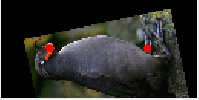
\includegraphics[scale=0.6]{img/wo_sym.png}
}
\quad
\subfigure{
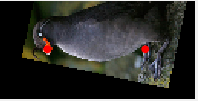
\includegraphics[scale=0.6]{img/w_sym.png}
}
%
\subfigure{
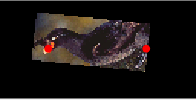
\includegraphics[scale=0.6]{img/ref_sym.png}
}
\caption{Illustration of the effect of the axial symmetry}
\label{fig:fig_sym}
\end{figure}


\section{Results}

\subsection{Birds Dataset}

First, we chose to evaluate the Poof method on the same dataset as in \cite{poof} to assess that our implementation is right. The Caltech-UCSD Birds 200-2011 dataset \cite{cud} contains 11,788 photographs of birds spanning 200 species. Each image is labeled with its species, a bounding box for the bird, and the image coordinates of fifteen parts: the back, beak, belly, breast, crown, forehead, left eye, left leg, left wing, nape, right eye, right leg, right wing, tail, and throat. The images are split into training and test sets, with about 30 images per species in the training set, and the remainder in the test set.\\

We ran our end-to-end process with the ground truth parts annotation on all the images for 7 parts up to 6 classes for computational limitations reasons. We computed the accuracy of our classifier and reported it in the figure \ref{fig:fig_acb} with regards to the number of classes. We reached an accuracy of around 90\%. This result is to compare to the 85.68\% in \cite{poof} on the whole 200 classes. Even though our accuracy is stable for the number of classes we consider, it may decrease if we consider a large number of classes.\\

\begin{figure}[H]
	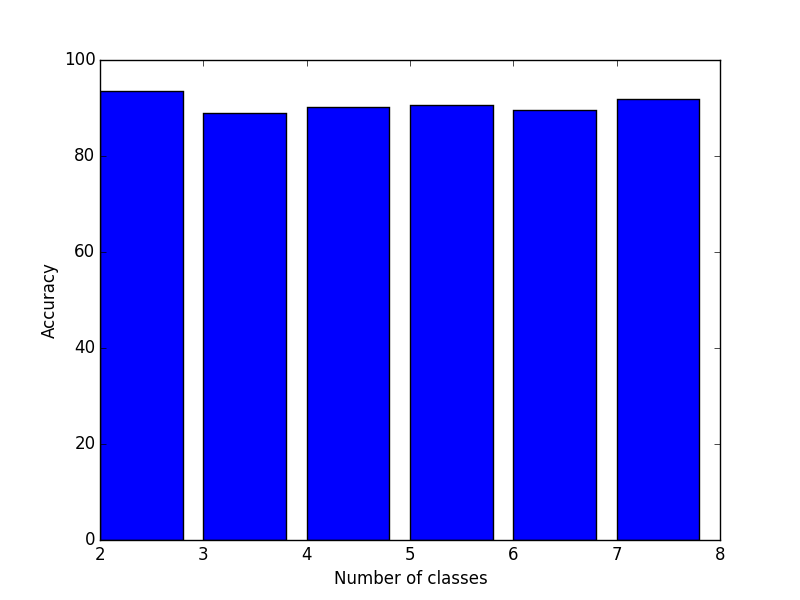
\includegraphics[scale=0.35]{img/acc_b.png}
	\centering
	\caption{Accuracy on the Birds dataset}
	\label{fig:fig_acc_b}
\end{figure}


This evaluation on the bird dataset confirms that our implementation is accurate and can be tested on other dataset.

\subsection{Whales Dataset}

For this dataset, we first present the results of our investigation on the parts annotation. Then, we decompose the Poof learning process to evaluate how well it performs on these images. Last, we provide accuracy results.\\

The whales dataset provided by Kaggle contains 11 500 images of 500 whales, 4500 are labelled and the question is to infer the identity of the whales on the 7 500 test images. The images are raw pictures taken by scientist with a normal camera over the course of 10 years and hundred of helicopter trips.A first observation is that the whale is most of the time hard to recognize even with the naked eye.\\

Different elements may perturb our work:
\begin{compactitem}
	\item Variable lighting conditions;
	\item Irregularities of the foam and of the water reflection over the different pictures;
	\item The orientation and position of the whale impacts the visibility of the features, for instance the whale can be covered by water.
\end{compactitem}

We work on images already croped with a bounded box around the nose, this script was provided on the Kaggle forum. This part of the work is done by Leonhard Spiegelberg.

\paragraph{Parts annotation}

This paragraph focuses on the main difference between the two dataset used and hence on one of the largest remaining challenge before being able to submit a result for the competition. As explained in the Poof process, we need pictures annotated with parts location as inputs. As a result, we need to find an automatic way to find this part in the whales dataset.

We first tried different feature descriptors to retrieve the interest points from the picture and then to match them among different pictures. The HARRIS features used to detect corners where tried but performed really poorly as soon as the whales are not almost the same as we can see in th figure \ref{fig:fig_haaris} The SIFT implementation provided by vlfeat \cite{vlf} performs well only when the nose is well observable. In the figure \ref{fig:fig_sift}, we observe a very good correspondences matching for two similar picture of the same whale. We can notive that this provides us interesting insights on possible interests points. But on the other pictures, the results are quite random. The bad quality of the entries makes it inefficient to solve our problem.


\begin{figure}[H]
\centering
\subfigure{
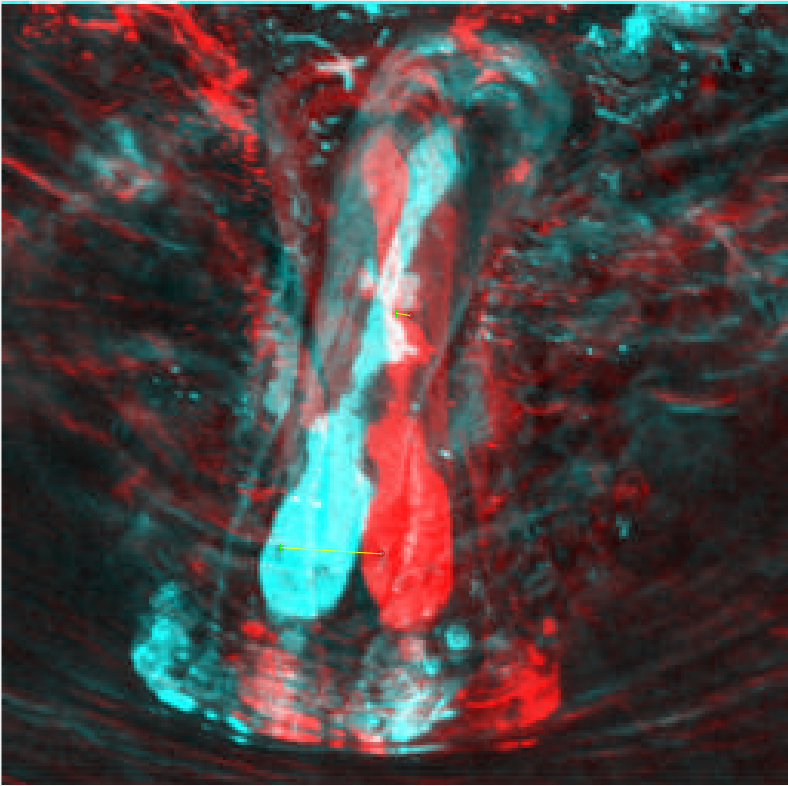
\includegraphics[scale=0.13]{img/haar_good.png}
}
\quad
\subfigure{
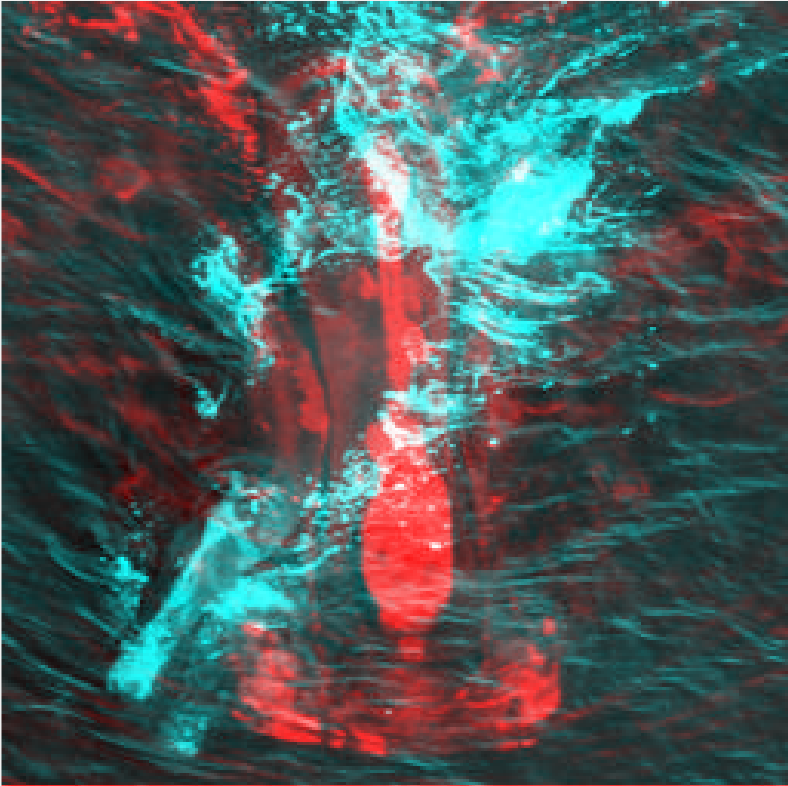
\includegraphics[scale=0.13]{img/haar_bad.png}
}
\caption{Matching provided with the HARRIS features}
\label{fig:fig_sift}
\end{figure}

\begin{figure}[H]
\centering
\subfigure{
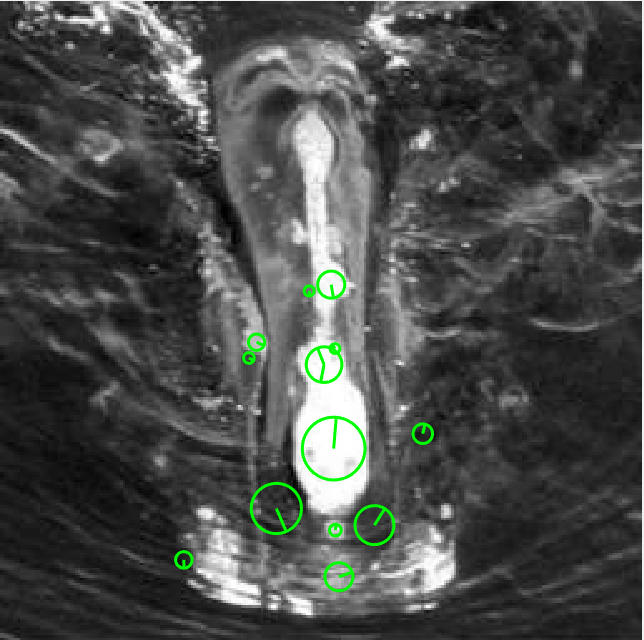
\includegraphics[scale=0.13]{img/corr_good.png}
}
\quad
\subfigure{
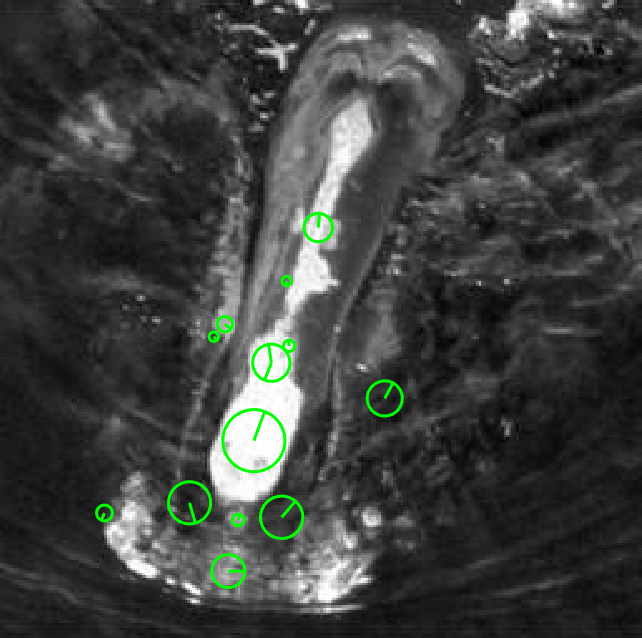
\includegraphics[scale=0.13]{img/corr_good_bis.png}
}
%
\subfigure{
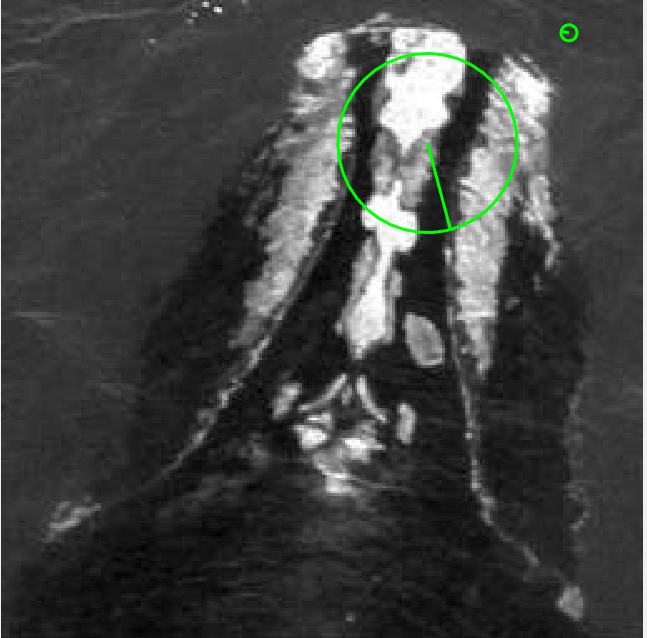
\includegraphics[scale=0.13]{img/corr_mid.png}
}
\quad
\subfigure{
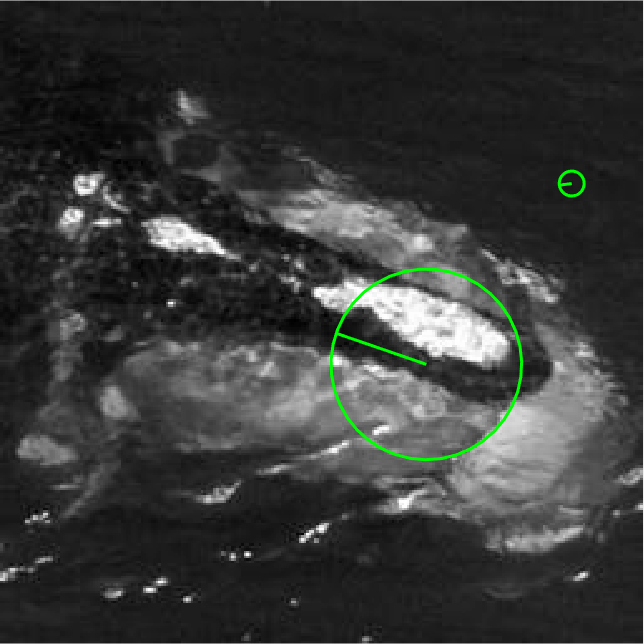
\includegraphics[scale=0.13]{img/corr_mid_bis.png}
}
\subfigure{
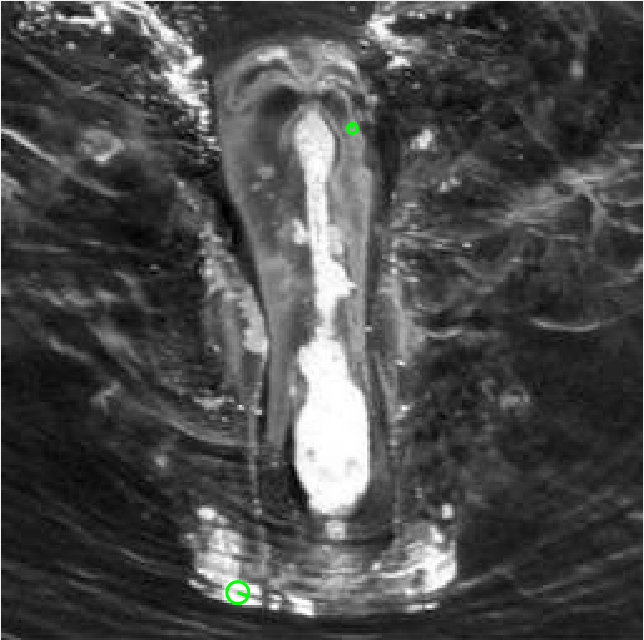
\includegraphics[scale=0.13]{img/corr_bad.png}
}
\quad
\subfigure{
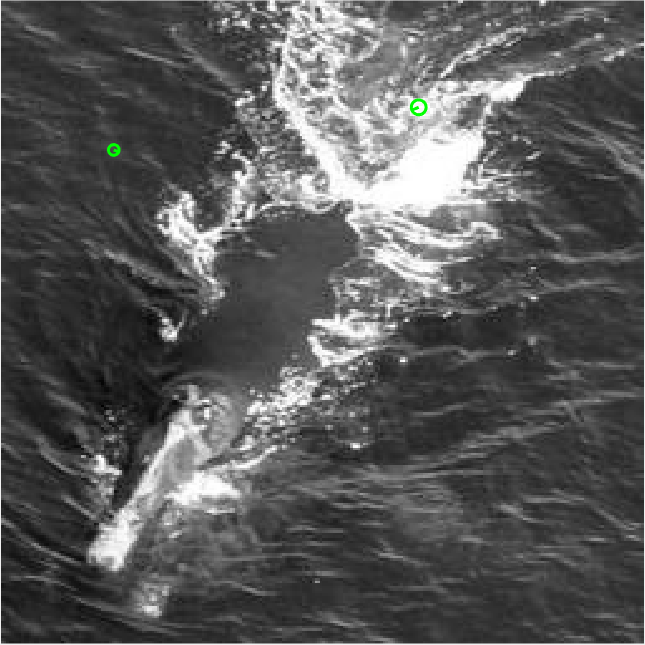
\includegraphics[scale=0.13]{img/corr_bad_bis.png}
}
\caption{Matching provided with the SIFT descriptor}
\label{fig:fig_sift}
\end{figure}



I manually annotated 120 pictures on 5 parts: the two extremities of the nose callosity, its middle point (which is relevant to differentiate the whale with a broken or a continous callosity) and the center of the two mandibulars. The first three parts are visible on all the picture. After several experiments, we observed that the best accuracy is reached if we consider only the three first parts.

\paragraph{Poof Process}

The first steps of the poof to align the images does not present any additionnal difficulties with the whales dataset:

\begin{figure}[H]
\centering
\subfigure{
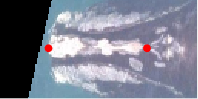
\includegraphics[scale=0.5]{img/std.png}
}
\quad
\subfigure{
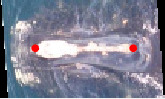
\includegraphics[scale=0.5]{img/std1.png}
}
\caption{Alignement and standardization of the images}
\label{fig:fig_std}
\end{figure}

Then, the HOG features are easily extracted with the vlfeat library. Even though, they manage to catch the shape of the callosities, it seems not so likely that a high difference may be observed for two different whales. An additional low level feature may help to grasp the nuances.

\begin{figure}[H]
\centering
\subfigure{
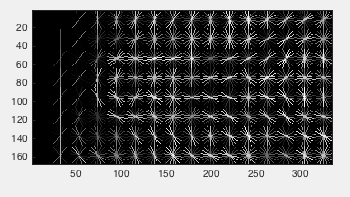
\includegraphics[scale=0.35]{img/hog1.png}
}
\quad
\subfigure{
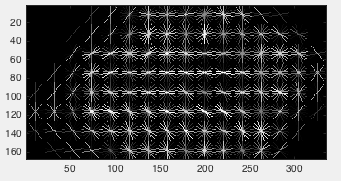
\includegraphics[scale=0.35]{img/hog2.png}
}
\caption{HOG features for the 2 considered tilings}
\label{fig:fig_std}
\end{figure}

The connected components selected after the thresholding on the weights assigned by the SVMs seem to change a lot from one class to another on the whales dataset. With the birds dataset, the component was most of the time well structured and relevant. Here, it seems to be more random. A solution to increase the robustness of the Poof approach even though some components may lack of structure could be to increase the number of parts considered to average the error provided by the bad components. This remains dependent on the automatisation of the annotation.

\begin{figure}[H]
\centering
\subfigure{
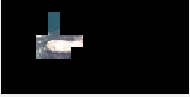
\includegraphics[scale=0.45]{img/cc_good.png}
}
\quad
\subfigure{
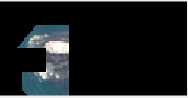
\includegraphics[scale=0.45]{img/cc_good1.png}
}
\subfigure{
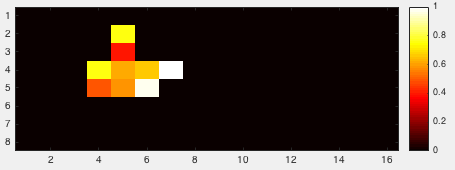
\includegraphics[scale=0.22]{img/weight_good.png}
}
\quad
\subfigure{
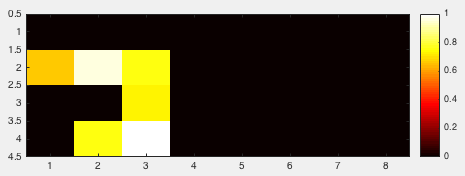
\includegraphics[scale=0.22]{img/weight_good1.png}
}
\caption{Connected components of average quality in the POOF process with associated weighs}
\label{fig:fig_std}
\end{figure}

\begin{figure}[H]
\centering
\subfigure{
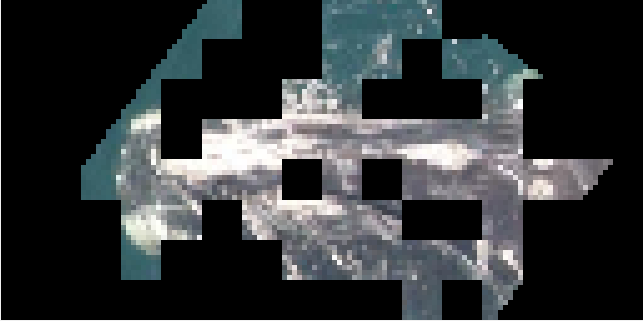
\includegraphics[scale=0.15]{img/cc_tile8_a.png}
}
\quad
\subfigure{
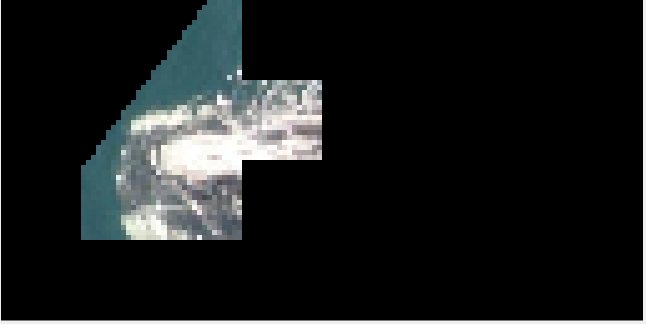
\includegraphics[scale=0.15]{img/cc_tile16_a.png}
}
\subfigure{
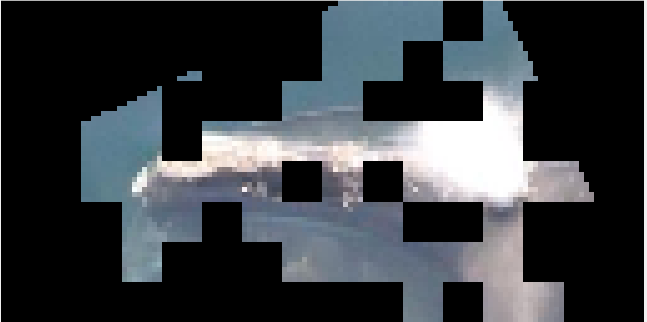
\includegraphics[scale=0.15]{img/cc_tile8_b.png}
}
\quad
\subfigure{
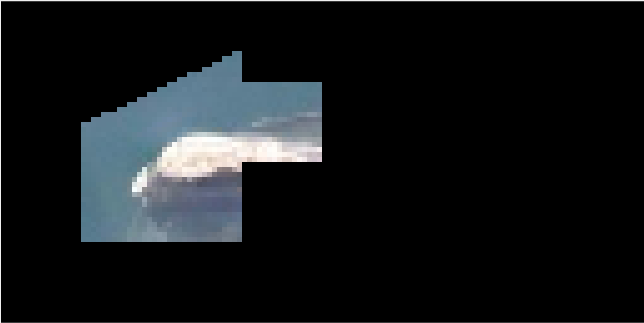
\includegraphics[scale=0.15]{img/cc_tile16_b.png}
}
\subfigure{
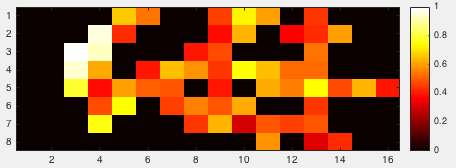
\includegraphics[scale=0.22]{img/weight_8.png}
}
\quad
\subfigure{
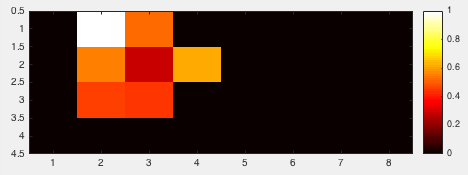
\includegraphics[scale=0.22]{img/weight_16.png}
}
\caption{Connected components of low quality in the POOF process with associated weighs}
\label{fig:fig_std}
\end{figure}

\paragraph{Classification accuracy}

We tested the model up to 4 different classes with about 25 images per class. We split the set in two equal parts for each class corresponding to the train and test test. We then evaluate the accuracy on the test set. The results are not as good as with birds. This is due to the lack of parts location information but also to the abd quality of the picture.

\begin{figure}[H]
	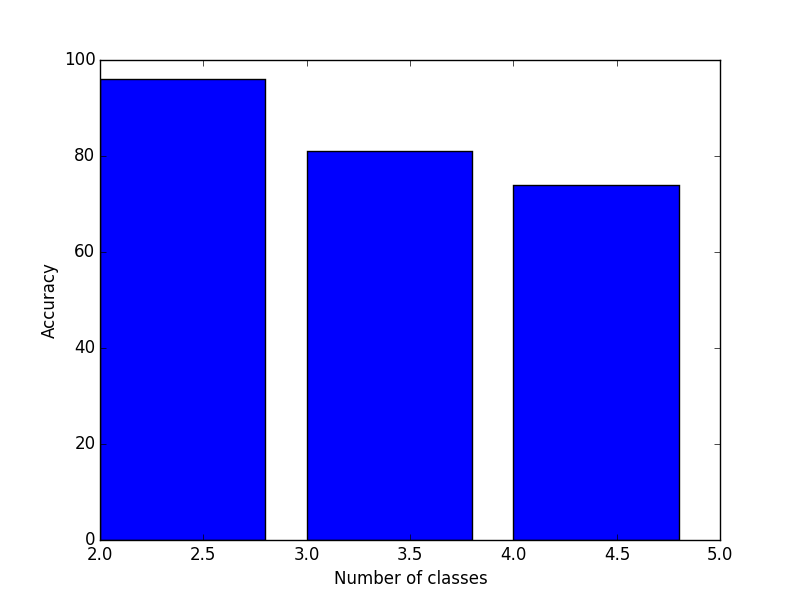
\includegraphics[scale=0.35]{img/acc_w.png}
	\centering
	\caption{Accuracy on the whales dataset}
\end{figure}



\section{Remaining Challenges}

Besides the need to find an automatic way for the parts annotations, we still have some remaining challenges. First, learning the Poofs for all the possible configuration when we have to deal with a large number of classes can be expensive in term of computational power. T. Berg used a sample of the possible configuration which still contained 5 000 features. The current matlab code may take around one to two weeks to learn these features. We could transpose the code into C++ or Python using OpenCv to take advantage of the parallelisation over GPU. This approach is really efficient for image processing as we have multiples simple operations to compute to build the features.\\

Another challenge specific to the whales dataset is the high skewness for some classes. We worked with classes of around 30 representants but the average number of representants per class is around 10, and some whales appear only on one or two pictures. This is a large issue because the SVMs learned will not be able to generalize well to the test entries for this class. 

\section{Improvement}

Even though we have remaining challenges, there are still many possibilites to improve the performance of our model. First, we could build an additional set of Poof features based on another low level feature, for example the color histogramm used by T. Berg. This could help to grasp the difference of callosities from one whale to another as their size is directly related to the white distribution on the picture.\\

Moreover, once we accumulate more annotated picture we could learn the similarities between the classes and then classify our entries using one-vs-most classifiers as suggested in \cite{snap}. This will help us to learn better the specific elements of each class because if really similar whales are present in the test set then these features are down weighted by the SVMs.

Lastly, we could introduce a preliminary step in our process where we remove the foam and the water refraction. This step could even provide only the whale after removing the water around with a background detection algorithm.

\section{Conclusion}

\noindent We implemented an end-to-end process functionnal on any kind of data set using the Poof method. Nonethelless, inputs with labeled and parts annotated images are required. This first work confirms the accuracy of this method on manually annotated image. The end-to-end process needs now to be extend with an automatic way to find the parts locations to fit the scope of our initial problem. Another approach could also be experiment using CNNs to have as inputs only labeled images.

%----------------------------------------------------------------------------------------
%	REFERENCE LIST
%----------------------------------------------------------------------------------------

\nocite{*} % Insert publications even if they are not cited in the poster
\bibliographystyle{unsrt}
\bibliography{sample}
\end{multicols}

\newpage


\end{document}



%----------------------------------------------------------------------------------------

